This chapter contains a brief overview inclusive description and definition of various inter-case resource dependency visualizations. First of all, in this context resources are described as durable resources, i.e resources that are assigned and released from events, but are neither destroyed or created.

\section{Resource Workload}
This section discusses several resource workload related visualizations. Resource workload is defined as the amount of events a resource is working at simultaneously for a certain point of time. This is a continuous value over time for each resource. Equation \ref{def:workload} defines the workload for a certain resource $r$ for time $t$, where $t \in l_T$. $l_T = \{\#_t(e) | e \in l \}$ being the set of all timestamps in event log $l$ and $E \in l$ being all events in event log L ordered ascending by $\#_{ts}(e)$ , i.e. chronologically by start date. The notation used in this thesis for selecting an event, case and log attributes it the following: $\#_{attribute}(object) = value$ and defined by \cite{aalst2016process}.

The sets $se$ and $ce$ are defined as a set of activity life-cycle transitions which denote the start and completion of an activity life-cycle, respectively. $\#_{ts}(e)$ denotes the time of the first occurrence of a start activity life-cycle transition for event instance $e$. Similarly, $\#_{te}(e)$ denotes the time of the last occurrence of a completion activity life-cycle transition for event instance $e$. Furthermore, $\#_{ts}(c)$ and $\#_{te}(c)$ denote the case start and end times, i.e. the time when the first event of the case was started, and the time when the last event of the case ended. The same applies for $\#_{ts}(l)$ and $\#_{te}(l)$ for the event log $l$. Note that the time dimension is simplified to be a discrete variable starting from $0$ for the first timestamp which is similar to \cite{aalst2016process}. The exact timestamp is not of importance in this context, only the relative time difference which can be illustrated in the simplified discrete setting.  

\begin{equation}\label{def:workload}
  \begin{array}{l}
    workload(r,t) =  
    | \{e \in l | \; \#_{ts}(e)  \leq t \leq \#_{te}(e) \wedge \#_r(e)=r\}| \; 
  \end{array}
\end{equation}

% \begin{figure}[h]
% 	\centering
%     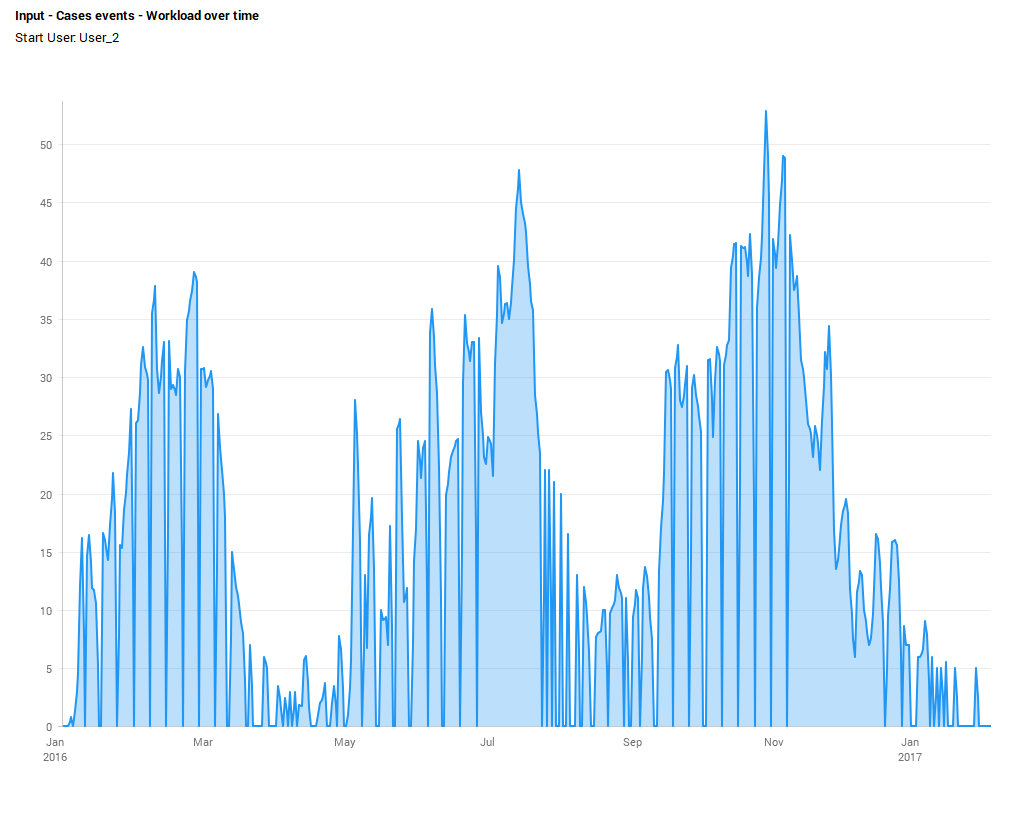
\includegraphics[width=.8\textwidth]{figures/workload.png}
%     \caption{Workload over time for User\_2 of the BPI Challenge 2017 event log.}
%     \label{fig:workload}
% \end{figure}

\begin{figure}[h]
	\centering
    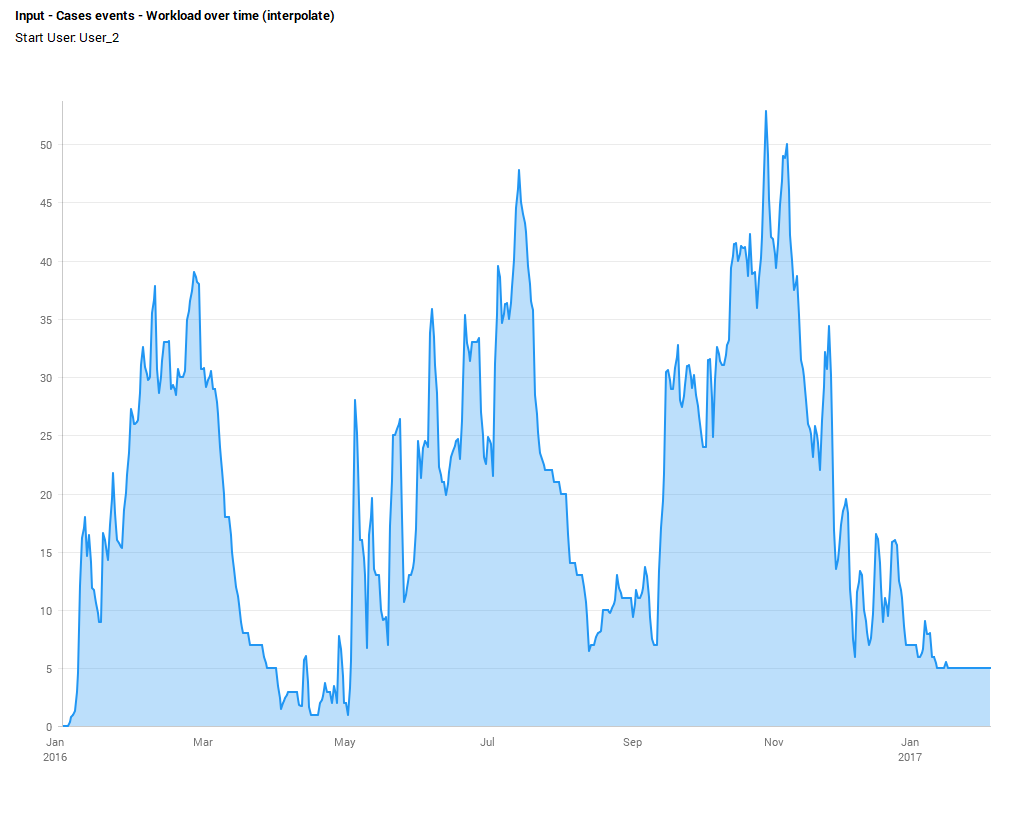
\includegraphics[width=\textwidth]{figures/workload_interpolate.png}
    \caption{Workload over time for User\_2 of the BPI Challenge 2017 event log.}
    \label{fig:workload}
\end{figure}

Figure \ref{fig:workload} illustrates the workload over time of the resource User\_2 for the complete period of the event log. The workload varies from fifty-three events to zero events. 

% The figure also shows a lot of downwards spikes to zero. This is because equation \ref{def:workload} returns zero when no events are performed by a resource for a specific period (in the case of Figure \ref{fig:workload}, the workload is calculated per day). However, this is incorrect, because the workload does not decrease to zero when no events are performed. Instead, the workload remains equal when no events are performed, i.e. the last non-zero workload value should be used. This is shown for the same data in Figure \ref{fig:workload_interpolate}. Equation \ref{def:amount} counts the number of events for a resource in a certain period and Equation \ref{def:workloads} simply returns all periods of minimal size of an event log.

% \begin{equation}\label{def:amount}
%     count(r,t_s,t_e) =  | \{e \in E | t_s \leq e_t \leq t_e \wedge e_r=r\}|
% \end{equation}

% \begin{equation}\label{def:workloads}
%     workloads(r) =  \{workload(r,t_s,t_s+1) | t_s \in t\}
% \end{equation}

% \begin{equation}\label{def:workload_interpolated}
%   \begin{array}{l}
%     workload\_in(r,t_s,t_e) =  
%     \begin{cases}
%     	workload(r,t_s,t_e) & \quad \text{if }  count(r,t_s,t_e) > 0 \\
%         workloads(r)_n \; s.t. \; \forall m \in t, m \leq n \wedge workloads(r)_m \leq t_s & \quad \text{if }  count(r,t_s,t_e) = 0
%     \end{cases}
%   \end{array}
% \end{equation}

\subsection{Resource Workload per Case}
In order to correlate the resource workload with case-specific variables, such as case outcome, it is necessary to calculate the average workload of users during a case execution. Equation \ref{def:workload_case} calculates the average workload of a single resource during a case execution by simply calculating all workloads and dividing by the number of workloads. Note that the workload is calculated for all points in time during the case execution. 

\begin{equation}\label{def:workload_case}
    avg\_wl\_during\_case\_resource(c, r) = \cfrac{\sum_{t=\#_{ts}(c)}^{\#_{te}(c)} workload(r,t)}{\#_{te}(c)-\#_{ts}(c)}
\end{equation}

Finally, Equation \ref{def:workload_case_resources} averages all the workloads for each resource working on the case, thus resulting in the overall average of the average workload for all resources during case execution. This overall average can give an indication of how busy the resources are during the case and might be used to correlate it with other variables such as case outcome. The latter is described in the next section. Note that $res(c)$ is defined as $res(c) = \{\#_{r}(e) | e \in c\}$ and $res(l) = \bigcup_{c \in l} res(c)$ for case $c$ and event log $l$, respectively. The methods simply return all resources which are associated with a case or log. 

\begin{equation}\label{def:workload_case_resources}
     avg\_workload\_case(c) = \cfrac{\sum_{r \in res(r)} avg\_workload\_case\_resource(c, r) }{|res(c)|}
\end{equation}

\subsection{Correlating Variables to Resource Workload}
This section elaborates on the previous sections by correlating the average case workload of all resources against other variables. An interesting correlation might be to correlate the average workload against the case outcome. For the BPIC 2017 dataset, which is about loan requests, the case outcome is either: \textit{success} when the loan request is accepted, \textit{denied} when the loan request is denied, \textit{cancel} when the loan request is either cancelled or the customer/bank did not reply in time or \textit{error} when no other outcome applies. The latter can occur because the case is not correctly closed due to administrative issues, or the case is not yet finished.

\begin{figure}[h]
	\centering
    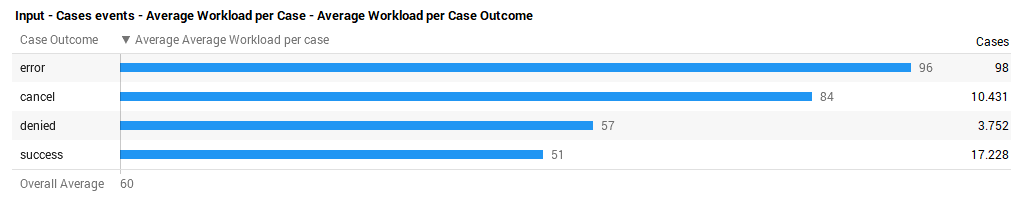
\includegraphics[width=\textwidth]{figures/workload_case_outcome.png}
    \caption{Average workload for each case outcome}
    \label{fig:workload_case_outcome}
\end{figure}

Figure \ref{fig:workload_case_outcome} shows the average workload with respect to case outcome. The average workload is calculated by simply averaging all case workloads with a certain outcome as is defined in Equation \ref{def:workload_case_outcome}. Figure \ref{fig:workload_case_outcome} shows a correlation between low average workload and successful loan request outcomes. Higher average workloads are correlated with denied and cancel outcomes (and error, but the amount of cases is relatively low). This could imply that when resources are very busy, i.e. have a high workload, the probability is higher than a case is cancelled. This might be the case because e.g. the resources do not have time to respond quickly so the customer in time so the customer finds another bank for their loan request.  

\begin{equation}\label{def:workload_case_outcome}
     avg\_workload\_case\_outcome(outcome) = \cfrac{\sum_{\{c \in l | \#_{outcome}(c)=outcome\}} avg\_workload\_case(c) }{|\{c \in l | \#_{outcome}(c)=outcome\}|}
\end{equation}

\begin{figure}[h]
	\centering
    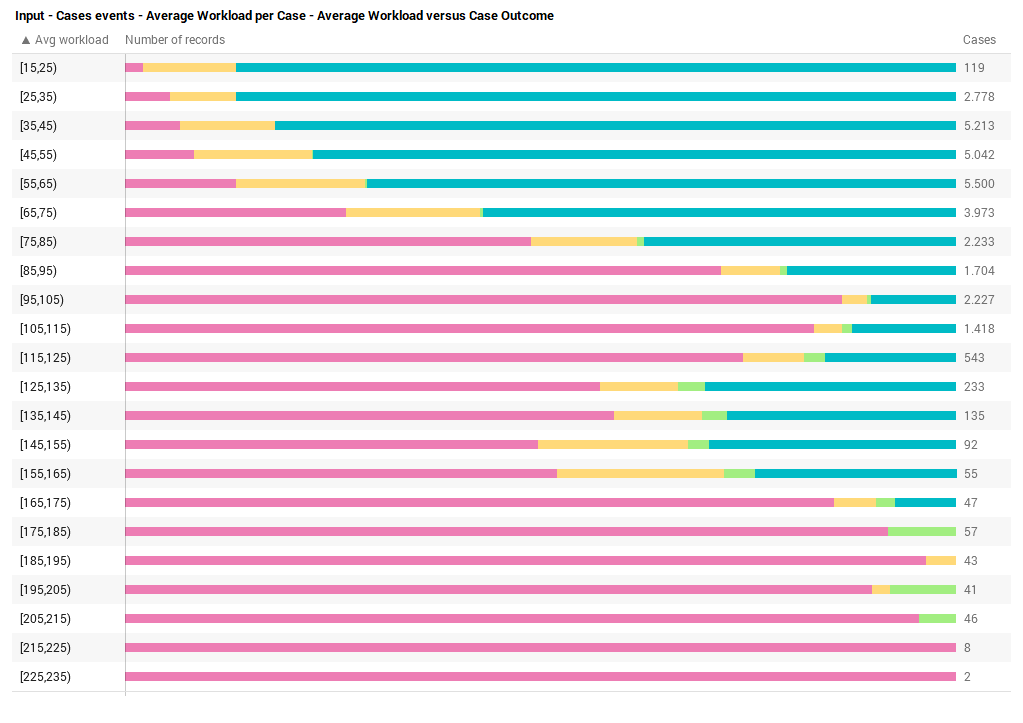
\includegraphics[width=\textwidth]{figures/workload_groups_case_outcome.png}
    \caption{Average workload with respect to case outcome}
    \label{fig:workload_groups_case_outcome}
\end{figure}

Figure \ref{fig:workload_groups_case_outcome} elaborates on Figure \ref{fig:workload_case_outcome} by splitting the cases into groups of average workload and showing the relative amount of case outcomes. The case outcome is shown in colours, whereas red represents \textit{cancel}, yellow represents \textit{denied}, green represents \textit{success} and light-green represents \textit{error}. The Figure shows that there is a clear connection between higher workload and higher relative size of \textit{cancel} outcomes.

It is very interesting that this trend does not completely hold because of the workload 125 until 165. This might however be an instance of the Yerkes–-Dodson law of arousal which indicates that there is a bell-shaped curved relation between workload and performance. More research is required in order to validate this.  

\subsection{Comparing workload between resources}

\subsection{Comparing workload between cases}

\section{Performance}
This section describes the performance metric for resources. the first section describes definitions which are used in the visualizations of the second section. 

\subsection{Definition}
The performance metric is defined for a certain resource for a certain point in time $t$. The performance measure simply counts the number of events which an employee completes on a point in time and is defined in Equation \ref{def:performance}. Note that trivially $\#_{ts}(l) \leq t \leq \#_{te}(l)$ should be the case.

\begin{equation}\label{def:performance}
  \begin{array}{l}
    performance\_completed(r,t) = 
   | \{e \in l | \#_{te}(e) = t \wedge \#_{r}(e)=r \}| 
  \end{array}
\end{equation}

Because time is a continuous value, it might not make sense to limit the performance to only a single point in time. Therefore, Equation \ref{def:performance_period} defines the performance for a certain resource on a specific period where $t_s$ is the start of the period and $t_e$ is the end of the period. The Equation is simply a sum over the time period for Equation \ref{def:performance}. Note that it should be the case that $\#_{ts}(l) \leq t_s \leq t_e \leq \#_{te}(l)$.

\begin{equation}\label{def:performance_period}
  \begin{array}{l}
    performance\_completed\_period(r,t_s, t_e) = \sum_{t = t_s}^{t_e} performance(r,t)
  \end{array}
\end{equation}

Equation \ref{def:events_started} describes the opposite of Equation \ref{def:performance}, namely the number of events which are started and allocated to a specific resource $r$ on a certain period in time $t$. The length of the worklist in Equation \ref{def:worklist} is calculated, because the worklist contains all 'open', i.e. unfinished tasks, for a certain resource. Equation \ref{def:events_started_period} is similar to Equation \ref{def:performance_period} and again is simply the sum over a period of time which generates the number of started events for a period.

\begin{equation}\label{def:events_started}
  \begin{array}{l}
    performance\_started(r,t) =
   | \{e \in l | \#_{ts}(e) = t \wedge \#_{r}(e)=r \}| 
  \end{array}
\end{equation}

\begin{equation}\label{def:events_started_period}
  \begin{array}{l}
    performance\_started\_period(r,t_s,t_e) = \sum_{t = t_s}^{t_e} events\_started(r,t)
  \end{array}
\end{equation}

Finally, Equation \ref{def:workload_delta} describes the change in workload for a certain resource on a point in time. When the workload delta yields a positive value, the workload of a resource increases, whereas negative values imply that the workload of a resource decreases. Equation \ref{def:workload_delta} is a simply the difference between Equation \ref{def:events_started} and Equation \ref{def:performance}. Equation \ref{def:workload_delta_period} is again the sum over a period of Equation \ref{def:workload_delta}.

\begin{equation}\label{def:workload_delta}
  \begin{array}{l}
    workload\_delta(r,t) =  performance\_started(r,t) - performance\_completed(r,t) 
  \end{array}
\end{equation}

\begin{equation}\label{def:workload_delta_period}
  \begin{array}{l}
    workload\_delta\_period(r,t_s,t_e) = \sum_{t = t_s}^{t_e} workload\_delta(r,t)
  \end{array}
\end{equation}


\subsection{Visualization}
This section elaborates on the definitions of the previous section by using them in several visualizations. This section presents rather simple, yet useful visualizations for resource performance. 

Figure \ref{fig:tasks_started} illustrates the tasks started summed for all resources. The graph distinguishes automated and manual events. Automated events are defined as events which take less than thirty seconds or contain only an end activity life-cycle activity. The Figure shows that the automated events closely follow the manual events, i.e. for each manual event, multiple automated events are performed. Further investigation validates that this is indeed the case.   

The Figure shows a clear pattern which is distinctive for the BPI Challenge 2017 dataset. It appears that almost no events arrive during the weekends (which is not uncommon for banks due to their limited opening hours) and that the events stream starts on Monday. Figure \ref{fig:dayofweek} supports this assumption by showing the average difference between started events of a day compared to the previous day. The Figure clearly shows that on Monday, much more events are started than the day before. Tuesday until Friday are rather stable, meaning that not almost the same amount of events are started as on Monday. Thursday seems to have a small decrease in events compared to Wednesday. This means that the amount of events peak, on average, each Wednesday. As expected, in the Weekend, significant fewer events are started than during the week. 

\begin{figure}[h]
	\centering
    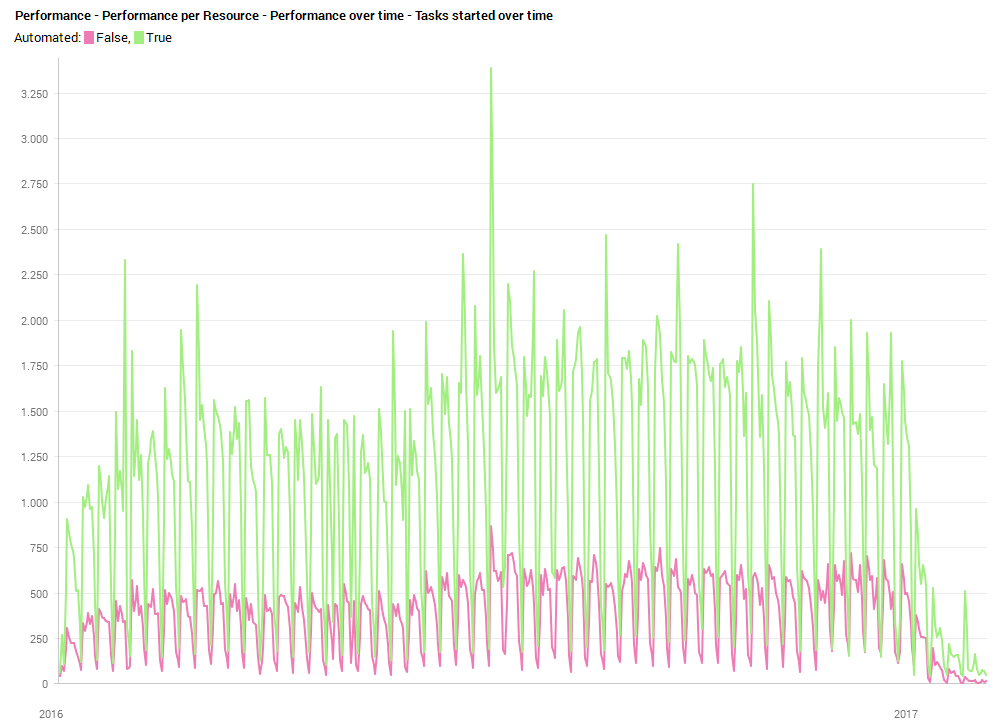
\includegraphics[width=0.9\textwidth]{figures/tasks_started.png}
    \caption{Tasks started over time for the BPIC2017 log.}
    \label{fig:tasks_started}
\end{figure}

\begin{figure}[h]
	\centering
    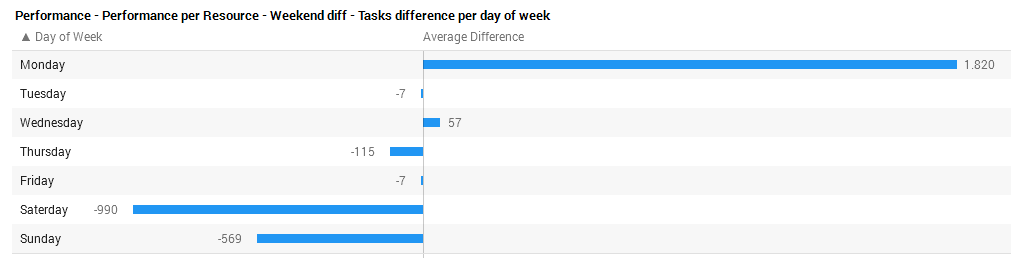
\includegraphics[width=0.9\textwidth]{figures/dayofweek.png}
    \caption{Average tasks started difference per weekday with respect to the previous weekday.}
    \label{fig:dayofweek}
\end{figure}

Figure \ref{fig:performance} shows a similar pattern as Figure \ref{fig:tasks_started} and describes the amount of events completed for each day. The Figures appear to closely follow each other, i.e. when more tasks are started, more tasks are completed. This could indicate that there is a sufficiently large pool of resources available which can handle all incoming cases. 

\begin{figure}[h]
	\centering
    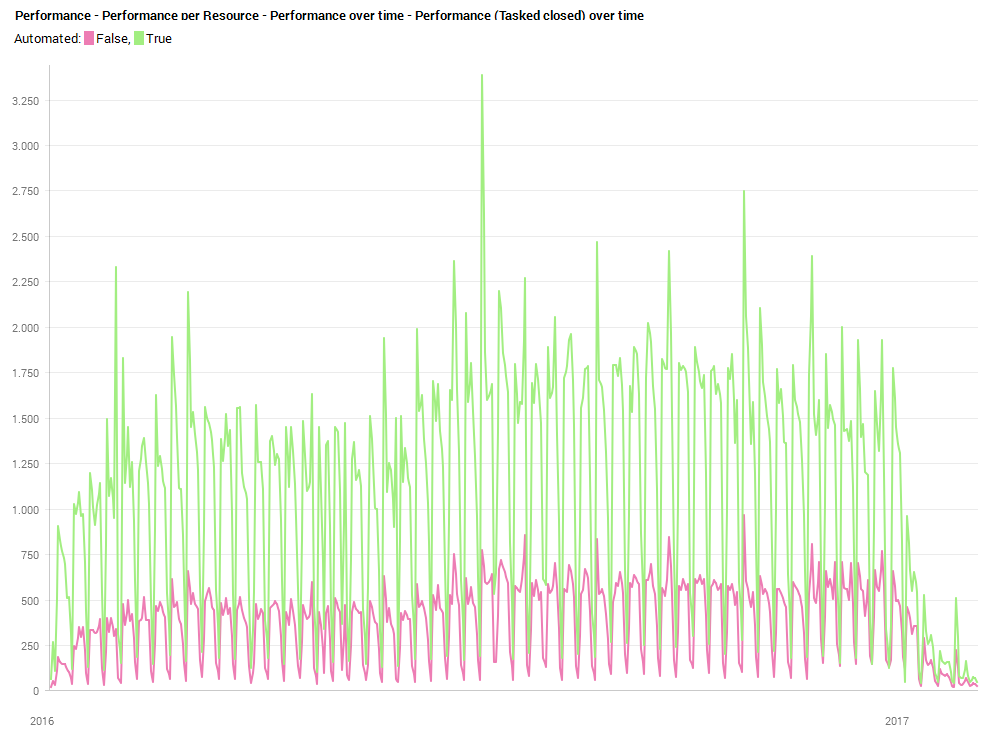
\includegraphics[width=0.9\textwidth]{figures/performance.png}
    \caption{Tasks completed (performance) over time for the BPIC2017 log.}
    \label{fig:performance}
\end{figure}

Figure \ref{fig:workload_delta} illustrates the difference between the tasks started and the tasks completed for all days. It shows that in general, the workload is rather stable, i.e. not many tasks are left open for a long time because after each positive spike, a negative spike occurs. This can be seen especially in the middle of the graph, where after a long period of positive workload delta values, a large negative correction occurs. Note that this is during the holiday period (June, July) and that the process might be handled differently than normally. 

At the beginning and end of the dataset, a large period of positive and negative workload delta appears. This is probably is because of the case filtering, namely: at January 2016, employees might be working on finishing cases of 2015 which are filtered from the log. The same appears at the end of the log, namely that employees might be already working on cases which arrive in 2017 but are also not part of the log. Finally, an interesting pattern is that at approximately the 21$^{st}$ of each month a large negative correction takes place. This might imply that during this date many events are completed using batch processing. 

\begin{figure}[h]
	\centering
    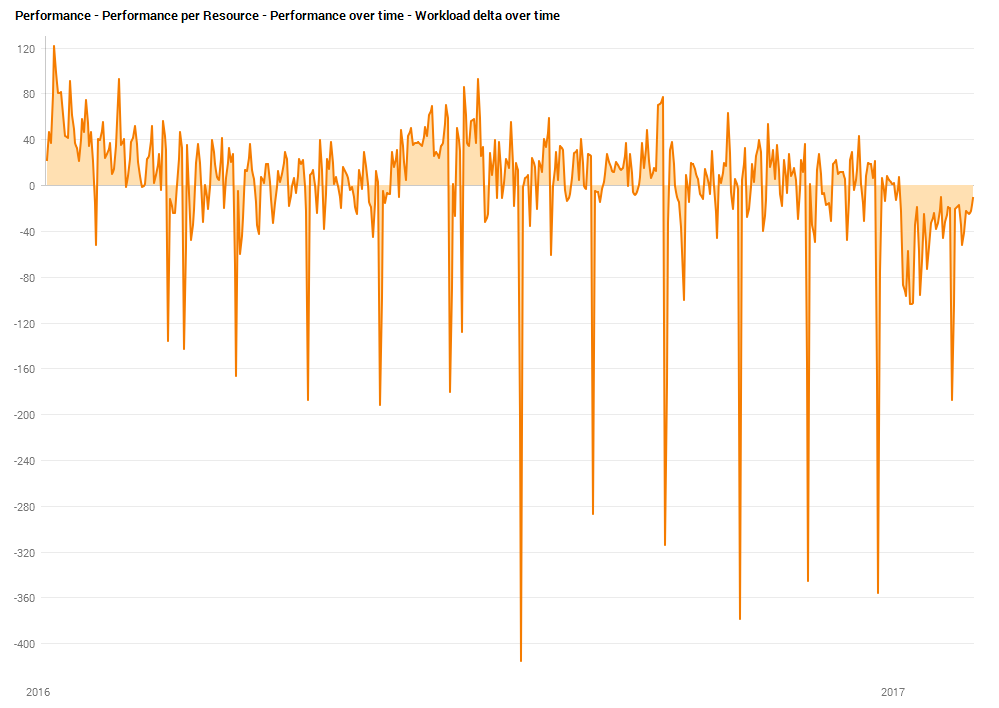
\includegraphics[width=0.9\textwidth]{figures/workload_delta.png}
    \caption{Workload delta over time for the BPIC2017 log.}
    \label{fig:workload_delta}
\end{figure}

\section{Resource Prioritization Policies}
This section discusses several prioritization policies visualizations. Prioritization Policies are general methods which resources can follow in order to define what their next task is. Resources each have a WorkList, which is an ordered queue of tasks which are allocated to a resource. WorkList $wl$ is ordered on arrival of tasks and contains all open (i.e. unfinished) tasks of a single resource. $\#_{wl}(r)$ denotes the WorkList of resource $r$. 

Each resource might use a different prioritization policy, or this policy might be fixed for certain groups of resources/departments. Either way, it might be interesting to analyse the which resource prioritization policy is used, and what effect it has on the process. The next section describes the definitions necessary for the visualization of the resource prioritization policies. The next section shows and describes the visualizations. 

\subsection{Definitions}

The first step is to calculate the WorkList at all points in time for each resource. This is important because the WorkList is the basis for calculating which resource prioritization policy is used. The $worklist(r, t)$ function requires a resource and a point in time, whereas $\#_{ts}(l) \leq t \leq \#_{te}(l)$. Equation \ref{def:worklist} describes this function. The function simply lists all events where $\#_{ts}(e) \leq t$, i.e. the events start before or on time $t$ where $t < \#_{te}(e)$, i.e. the events end after time $t$. In other words, it lists all open tasks at point $t$. This function is abbreviated to $wl(r,t)$.

\begin{equation}\label{def:worklist}
  \begin{array}{l}
    worklist(r, t) =  \{e \in l |\; \#_r(e) = r \wedge \#_{ts}(e) \leq t < \#_{te}(e)   \}
  \end{array}
\end{equation}

% Old recursive function
% \begin{equation}\label{def:worklist}
%   \begin{array}{l}
%     worklist(r, t) =  
    
%     \begin{cases}
%     worklist(r, t -1) + \{e \in E | e_r = r \wedge e_l \in se & \text{for } t \leq t_s \\ 
%      \wedge   e_t = t \} - \{e \in E | e_r = r 
%     \wedge e_l \in ee \wedge e_t = t\} \\ 
%     [ \; ], & \text{for } t < L_ts
%   \end{cases}
%   \end{array}
% \end{equation}

A method to see how much a certain resource follows a prioritization policy is to define a penalty function for all policies. The policy with the lowest penalty is then followed best. Equation \ref{def:fifo} defines the penalty function of FiFo and checks whether there exist events at all for time $t$, otherwise, the penalty is simply zero. Furthermore, it is checked whether the worklist has at least more than one item, otherwise, the penalty is also zero. The latter is the case that the penalty does not make sense when the worklist contains zero or one items because one cannot prioritize a single item. 

If there exist any events, the $fifo\_penalty(r,e)$ function is called for each event the results are summed up. Note that $wlr$ is defined as $wlr = wl(r, \#_{te}(e))$ The $fifo\_penalty(r,e)$ in Equation \ref{def:fifo_penalty} first checks whether the event exists in the workload (which should always be the case for non-automated events, otherwise an event has not been started, only completed), if not zero is returned. In all other cases, the FiFo penalty is defined as the size of the worklist minus the index of the event defined by the worklist size. The latter step is to normalize the error, otherwise, a high worklist might imply higher violations. The Equation shows a linear normalization, but other normalizations can also be considered. When the index is high, i.e. the event has just been added to the worklist, the penalty is lowest, while when the index is low, i.e. when many more events have been added after the event start, the penalty is high.     

\begin{equation}\label{def:fifo}
  \begin{array}{l}
    fifo\_error(r, t) = 
    
    \begin{cases}
    	0, & \text{for } \exists{e \in l} | \; \#_{te}(e) = t \wedge \#_r(e)=r \\
        \sum_{\{e \in l | \#_{r}(e)=r \wedge \#_{te}(e)=t \}} fifo\_penalty(r,e)  & \text{otherwise}
    \end{cases}
  \end{array}
\end{equation}


\begin{equation}\label{def:fifo_penalty}
  \begin{array}{l}
    fifo\_penalty(r, e) = 
    \begin{cases}
    	0, & \text{for } |wlr| \leq 1 \wedge e \in wlr  \\
        \cfrac{|wlr| - |\{w \in wlr\; \#_{ts}(w)  \leq \#_{ts}(e)\}|}{|wlr|}  & \text{for } |wlr| > 1 \wedge e \in wlr
    \end{cases}
  \end{array}
\end{equation}

The same can be done for the LiFo penalty, only slightly simpler. Equation \ref{def:lifo} is almost equal to \ref{def:fifo}, instead, Equation \ref{def:lifo_penalty} is called instead of Equation \ref{def:fifo_penalty}. The only difference between the latter two equations is that the penalty is calculated by simply finding the index of the event in the worklist of the corresponding resource. This has the opposite effect as the fifo penalty, such that the penalty is high when the index is high, i.e. the event has just been added, and is low when the index is low, i.e. many events are added after the event has been started. This is exactly the difference between FiFo and LiFo. 

\begin{equation}\label{def:lifo}
  \begin{array}{l}
    lifo\_error(r, t) = 
    
    \begin{cases}
    	0, & \text{for } \exists{e \in l} | \; \#_{te}(e) = t \wedge \#_{r}(e)=r \\
        \sum_{\{e \in l | \#_{r}(e)=r \wedge \#_{te}(e)=t\}} lifo\_penalty(r,e)  & \text{otherwise}
    \end{cases}
  \end{array}
\end{equation}


\begin{equation}\label{def:lifo_penalty}
  \begin{array}{l}
    lifo\_penalty(r, e) = 
    
    \begin{cases}
    	0, & \text{for } |wlr| \leq 1 \wedge e \in wlr  \\
        \cfrac{|\{w \in wlr|\; \#_{te}(w)  \leq \#_{ts}(e)\}|}{|wlr|}  & \text{for } |wlr| > 1 \wedge e \in wlr
    \end{cases}
  \end{array}
\end{equation}

Finally, the last prioritization policy is Shortest Task in Queue and requires a slightly different penalty function. Note that $\#_{td}(e)$ is defined as $\#_{td}(e)=\#_{te}(e)-\#_{ts}(e)$, i.e. the duration of event $e$. Equation \ref{def:shortenalty} requires the construction of an ordered list of event durations, whereas each event in the worklist has exactly one corresponding duration value (i.e. end time minus start time). This means that the lowest durations have the lowest index and thus also the lowest penalty. 

\begin{equation}\label{def:short}
  \begin{array}{l}
    short\_error(r, t) = 
    
    \begin{cases}
    	0, & \text{for } \exists{e \in l} | \; \#_{te}(e) = t \wedge \#_{r}(e)=r \\
        \sum_{\{e \in l | \#_{r}(e)=r \wedge \#_{te}(e)=t\}} short\_penalty(r,e)  & \text{otherwise}
    \end{cases}
  \end{array}
\end{equation}

\begin{equation}\label{def:shortenalty}
  \begin{array}{l}
    short\_penalty(r, e) = 
    
    \begin{cases}
    	0, & \text{for } |wlr| \leq 1 \wedge e \in wlr  \\
        
        \cfrac{|\{w \in wlr|\; \#_{td}(w) \leq \#_{td}(e)\}|}{|wlr|}  & \text{for } |wlr|> 1 \wedge e \in wlr\\
    \end{cases}
  \end{array}
\end{equation}

\subsection{Visualization}
This section elaborates on the definitions of the last section by showing several visualizations based on the definitions. Figure \ref{fig:error_total} shows the total error for the FiFo, LiFo and Shortest Job First scheduling policies for the BPIC 2017 dataset. The weekly spikes are a noticeable artefact for this dataset. It appears that resources acquire their workload on Monday of all cases which arrived during the weekend and work their way through the worklist during the week. At the end of the week, the worklists are almost empty and no tasks are performed during the weekend. This pattern can also clearly be seen in Figure \ref{fig:error_total}.

\begin{figure}[h]
	\centering
    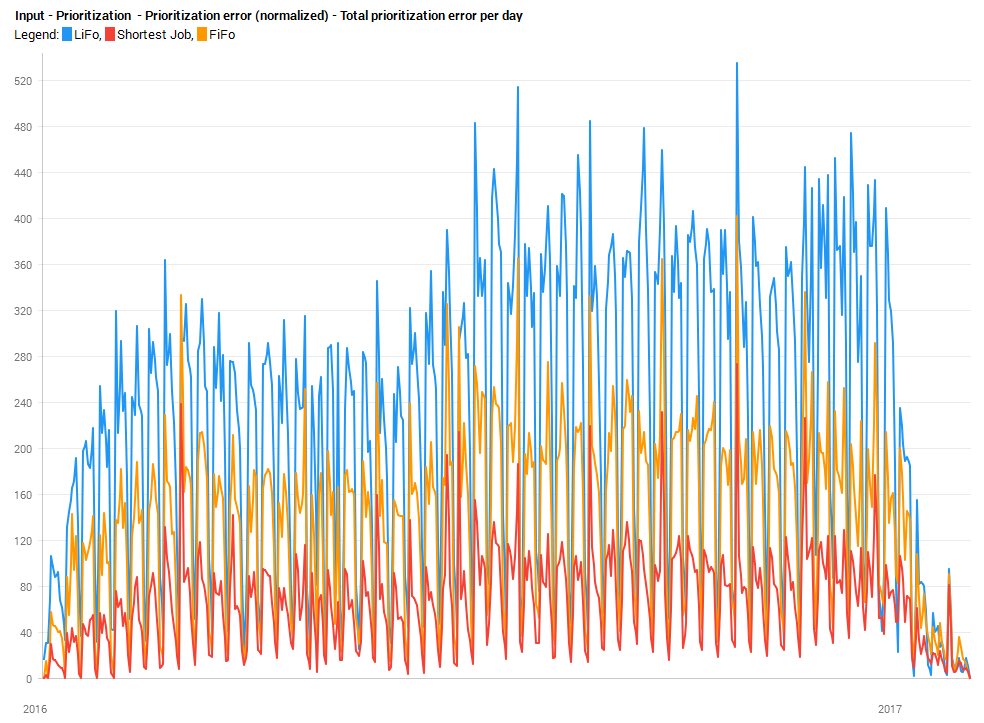
\includegraphics[width=0.9\textwidth]{figures/total_prioritization_error.png}
    \caption{Total FiFo, LiFo and shortest job error of BPIC2017 per day.}
    \label{fig:error_total}
\end{figure}

When inspecting the figure briefly, it can be seen that, on average, the LiFo penalty seems to be highest at most times, while the Shortest Job First error seems lowest at almost all times. The FiFo error is in between these two errors. This indicates that the prioritization is executed more accordingly to the Scheduled Job First policy, than according to the LiFo policy. Furthermore, one can notice no significant changes over time, expect at the begin and end of the log where there are sudden decreases and increases. This is however the effect of a case filter which removes all open cases in the event log. 

The average FiFo penalty is 0.044, and in 112,293 event instances, a FiFo penalty was given. Thus indicating that in these event instances FiFo was not fully followed. For LiFo, the average error is 0.074 and the amount of event instances with a penalty is 141,949. Compared to FiFo, LiFo has both a higher average error and more event instances which have a LiFo error. Thus indicating that the prioritization schedule is more likely to follow FiFo than LiFo. Finally, the average Shortest Job First penalty is 0.021507 and the amount of event instances which have a penalty is 89,650. Both values are significantly lower compared to LiFo and FiFo, thus indicating that this scheduling method might be a better fit. 


\begin{figure}[h]
	\centering
    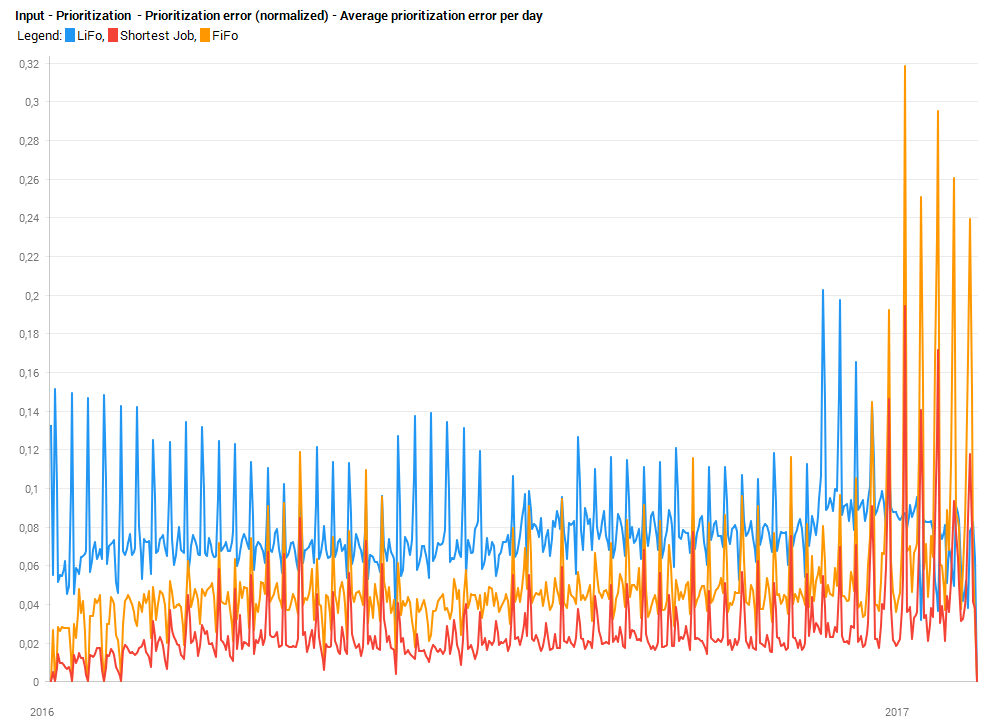
\includegraphics[width=0.9\textwidth]{figures/avg_prioritization_error.png}
    \caption{Average FiFo, LiFo and shortest job penalty of all events for BPIC2017 per day.}
    \label{fig:error_avg}
\end{figure}

Another way of visualizing the prioritization penalties is by taking the average penalty per event and is shown in Figure \ref{fig:error_avg}. This Figure contains the same finding as \ref{fig:error_total} that most of the time, the Shortest Job First policy seems to be followed best and the LiFo policy seems to be followed least. However, this Figure contains an interesting increasing trend at the end of the dataset, where the average LiFo error decreases and the Shortest Job First and FiFo policies significantly increase.  

Finally, Figure \ref{fig:error_avg_nnull} is similar to Figure \ref{fig:error_avg}, expect from the fact that only the non-zero penalties are taken into account. In other words: the Figure contains the average of all events which do not strictly follow the prioritization policy. This shows that, except the last months, the LiFo is close to the maximum of one, meaning that the LiFo scheduling policy is not followed at all. 

\begin{figure}[h]
	\centering
    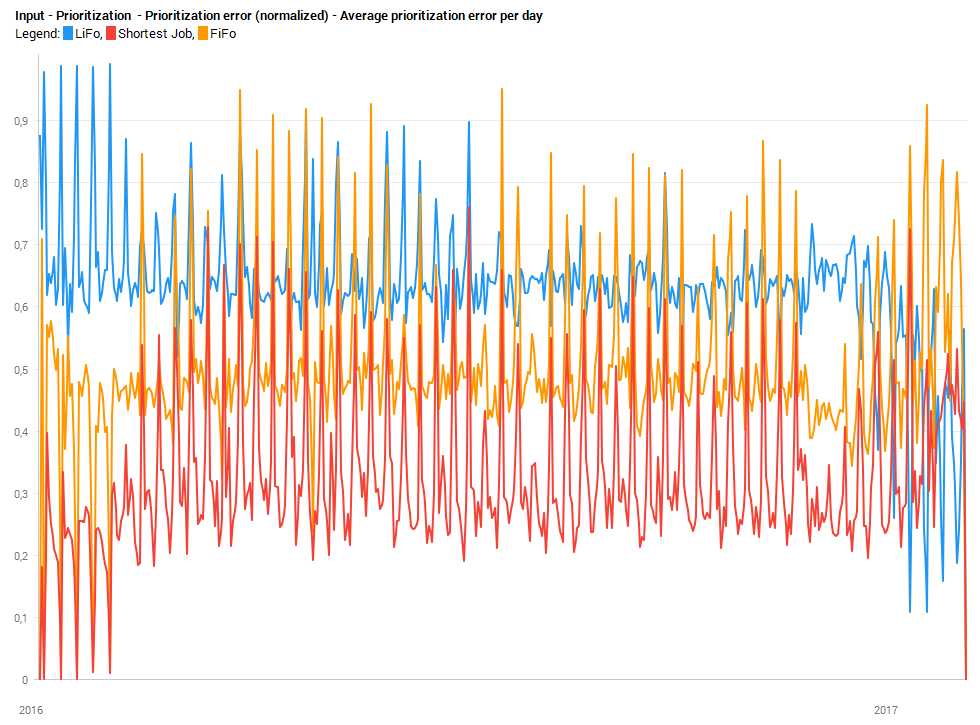
\includegraphics[width=0.9\textwidth]{figures/avg_error_nnull.png}
    \caption{Average FiFo, LiFo and shortest job penalty of all non-zero penalties for BPIC2017 per day.}
    \label{fig:error_avg_nnull}
\end{figure}

\section{Annotating Process Models}